\documentclass[border=2pt]{standalone}
\usepackage{pgfplots}
\pgfplotsset{compat=1.18}

\begin{document}

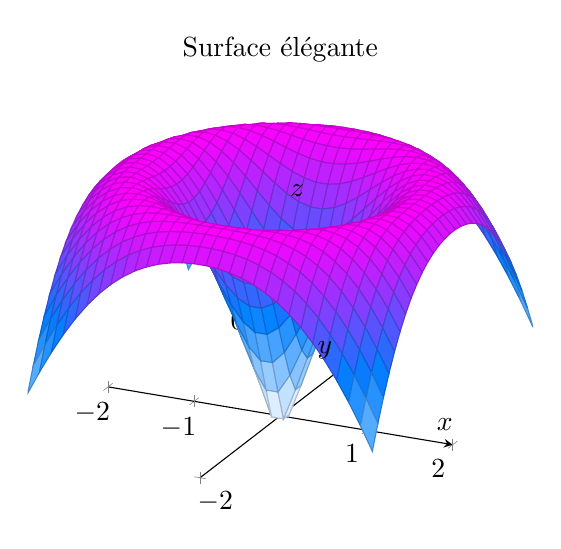
\begin{tikzpicture}
    \begin{axis}[ 
        axis lines=middle, 
        title={Surface élégante}, 
        xlabel={$x$}, ylabel={$y$}, zlabel={$z$},
        colormap/cool, % Choisir un colormap attractif
        grid=both, 
        width=8cm
    ]
        \addplot3[surf, domain=-2:2, y domain=-2:2, samples=30] 
        {sin(deg(sqrt(x^2 + y^2)))};
    \end{axis}
\end{tikzpicture}

\end{document}
